
\documentclass[a4paper,12pt]{article}

%% PACKAGES %%
\usepackage{graphicx,times,fancyhdr,algorithm,algorithmic,url}
\usepackage[left=1in,top=1in,right=1in,bottom=1in]{geometry}
\graphicspath{{./images/}}

%% DOCUMENT START %%
\begin{document}

% page numbers and headers
\thispagestyle{plain}
\pagestyle{fancy}
\clearpage
\setlength{\headsep}{0.4in}

\title{Viewed More\\ \large Measuring the effect of YouTube video title wording on view count}
%\title{Viewed More\\ \large Using NLP to Predict YouTube View Counts from Titles}
\date{\today}
\author{
  {\rm Erik Kessler and Greg Szumel}\\
  Williams College\\
  CSCI 375 \\
  Spring 2017
}

\maketitle

\lhead{CS 375}
\chead{Viewed More}
\rhead{Kessler, Szumel}
\cfoot{\thepage}

\begin{abstract}
We created a Naive Bayes classifier designed to predict whether a YouTube video is likely to receive more or less views than average for the uploader based on the title. Such a system would allow YouTube content creators to increase their view counts and would allow YouTube to increase traffic and user engagement. We created a dataset of 25k video titles from the top 1600 subscribed YouTubers. Our dataset is labeled based on the number of standard deviations away from the uploader's mean view count per video the video is. We created a variety of features including different collocational and co-occurance features as well as unigram and bigram features and capitalization and length features. We were able to achieve an F1 of 0.515, and our classifier works best we filter out videos from around the mean from our training set and when titles are keyword-based. 
\end{abstract}


\section{Introduction}
Every minute, hundreds of hours of video are uploaded to YouTube. How can YouTube content creators or uploaders stand out from the crowd and draw an audience to their videos? One tool they have at their disposal is the video title. Video creators try to make their videos sound enticing by putting a flashy and interesting title to spark interest and curiosity in users with the hope the user will choose to watch their video. View counts are not only a measure of popularity but are also the main currency of YouTube as more views correspond to more opportunities for advertisements. Therefore, video creators would be interested in improving their titles to earn more money and draw more subscribers to their channel. YouTube itself is interested in keeping users on their site by making sure users continue to see interesting titles and continue to click through to those videos.

\begin{figure}[h]
    \centering
    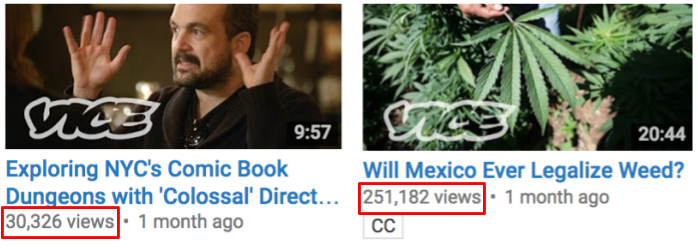
\includegraphics[width=.7\textwidth]{motivation}
    \caption{Two videos from the same uploader with drastically different view counts.}
    \label{fig:motivation}
\end{figure}

There would be value for both YouTube and video uploaders alike if when a creator uploaded a video, the site could indicate the quality of the title and even suggest a better title that would draw more views. The goal of this project was to develop a system that could predict how a video would do based on different features of the title. Such a system could also be used to filter interesting titles towards the top of search results or towards the top of a suggested videos page. Furthermore, this could be extended to detect video titles that go too far and cross into the category of clickbait which YouTube might want to filter out to avoid disappointing and annoying users.

\section{Related Work}
Our interest in this project was initially sparked by Chenhao Tan, Lillian Lee, and Bo Pang's project \textit{Retweeted More} \cite{tan+lee+pang:14}. In \textit{Retweeted More}, they developed an algorithm for predicting which of two tweets on the same topic would receive more retweets. They found that wording does matter. There are features that improve the probability that a tweet will be retweeted. This finding suggests that we will find features in YouTube title wordings that influence the number of views. We also predict that the features that improve YouTube titles will differ from those that improve tweets which is why we were interested in expanding on that project to explore YouTube. Furthermore, for this existing work, creating a dataset of content and author controlled tweets while also controlling for other confounding effects such as when the tweets were sent was a major component of the project and as they creatively used tweets-pairs from the same account linking to the same content but with different wordings as natural experiments. We would need to find or create a similar dataset for YouTube videos. \\

Existing work on determining which factors impact the popularity of YouTube videos have focused on factors such as social networks and view count histories \cite{youmna+ardon+carlsson+eager+mahanti:12}. It is difficult for a YouTuber to easily change the structure of their social network or their video's viewing patterns, so we wanted to focus on something that the uploader could easily adjust that would help them achieve more video views. Since we knew from Tan that wording had an impact on retweets and Borghol did not look at title wording, we realized we could add to existing research by studying the effect of title wording on view counts. Borghol also offered us a promising dataset of cloned videos which were sets of different re-uploads of the same video by different users. Unfortunately, many of the videos were non-English and those that were in English were movie trailers so they did not capture the types of videos on YouTube we wanted to explore. \\

Another piece of relevant work we looked at was Himabindu Lakkaraju's work on examining the effect of titles on the success of Reddit image posts \cite{himabindu+mcauley+leskovec:13}. Their finding that the title wording influences the success of a post further confirmed that wording matters, but research is missing on title wording on YouTube and what features make a good video title. Additionally, this work provides some starting points as the authors identify some linguistic features of titles that impact popularity. \\

Overall, out survey of existing work shows that wording matters, having a dataset that controls for possible confounding variables is important, and there is a current lack of literature on what features of YouTube video titles predict more popularity and views. We look to build off this existing work with our own study of wording effects on YouTube titles.


\section{Formulation}
We formulate our problem as a classification problem. We are looking to classify a string of words representing a title as either a ``good'' or ``bad'' title where good means the title will likely get more than average views and bad means the title will likely get fewer views than average. \\

To do the classification, we will construct a feature vector for the title using a variety of features that we think would be useful for predicting how a title would perform. We can then use a set of labeled feature vectors to train a classifier and use that classifier to predict the quality of unseen titles.

Because of our common sense and also findings by Lakkaraju, we know that the content of the video will affect the view-count. However, we want to hold as many variables constant as possible. In previous work, they were able to find duplicate tweets or images that had different titles. This simplified the classification problem so long as there were enough data points to determine which titles were better. This was why the clone-video dataset was especially promising. We believed we could use a similar approach as the retweeted more to determine which titles might be better. However, upon further investigation, we found that the videos were not all in English and were mostly trailers. The non-english trailers would deplete the number of videos in the dataset that we could actually use and we were concerned that because the videos were mostly trailers our product might be biased to only work for titles with 'trailer-ish' content. Even more, Lakkaraju also found they were unable to determine if differences between the videos were influenced by the user posting. This was especially problematic, where a heavily subscribed channel that posted a video would have a very high view-count for a particular title, but another one that might have a 'better' title would have a lower view count. For all of these reasons, we decided it best to try to standardize across channels.

Instead of using the limited clone dataset, we chose to use to top YouTubers' most recent videos. These, we believed, would be the most relevant to our question for a few different reasons. First, it solved the problem of channel viewer influence. Instead of looking at individual videos, we would look at a particular channel's videos, where we could standardize across the channel, ranking each title as either 'good' or 'bad'. Further, we hypothesized that other factors including thumbnail picture quality, which appears with the title, should also be fairly consistent across a channel. However, we do lose 'content' control. In the clone video dataset, content between videos was the same. Here, content is different, which introduces variability between different titles simply on the premise of content. 


\section{Architecture Overview}
Provide an overview of your system, presenting and justifying important design choices such as algorithms, features, etc.\\



We decided to impose two different restrictions on the data. First, we wanted to get rid of most Title's of songs, so we got rid of any VEVO titles, or any titles that had detectable song names in them. We thought that removing songs from our dataset was important, since those titles lacked the creativity and variability we were hoping to capture. In other words, YouTube videos with titles attached are simply the titles of the song with the artist's name attached. 

From there, we wanted to get rid of channels, or non-users. There were channels that included just \#MUSIC or \#POPULAR that we did not want in our dataset, so we decided to remove all channels from our dataset. 


\begin{figure}[h]
    \centering
    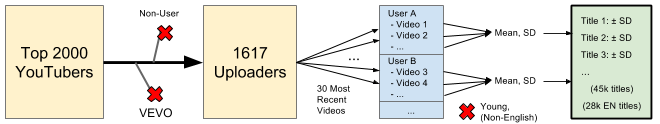
\includegraphics[width=.99\textwidth]{dataset}
    \caption{Diagram showing the dataset creation process resulting in 45k total titles and 28k English titles.}
    \label{fig:dataset}
\end{figure}

Then, we wanted to rank each video as either a good video or a bad video, per channel. So for each channel, we calculated the mean and the standard deviation of the view counts. We labelled any video that had a positive standard deviation count as a "GOOD" video, and any video that had a negative standard deviation count as a "BAD" video. The counts of videos after this filtering is listed below. 

We then split the two data sets into English only groups and Universal groups, where we filtered any non-English title out in the English only section. However, the program doing this was not entirely accurate, so some videos in the group are not English, but these videos are limited in number, and we believed would not play a significant role in title detection. But to safeguard against poor English results, we created the Universal group, which did not filter by language. 

\begin{table}[h]
  \small
  \centering
  \begin{tabular}{|l|l|l|l|}
    \hline
    \textbf{Universal}&&& \\ \hline \hline
    \textit{Use} & \textit{SD Thresh.} & \textit{GOOD} & \textit{Total} \\ \hline 
    Test & 0.00 & 4741 & 13625 \\ \hline
    Train & 0.00 & 11148 & 31789 \\ \hline
    Train & 0.25 & 8533 & 24812 \\ \hline
    Train & 0.50 & 6652 & 15725 \\ \hline
  \end{tabular}
  \quad
  \begin{tabular}{|l||l|l|l|}
    \hline
    \textbf{English-Only}&&& \\ \hline \hline
    \textit{Use} & \textit{SD Thresh.} & \textit{GOOD} & \textit{Total} \\ \hline 
    Test & 0.00 & 2869 & 8400 \\ \hline
    Train & 0.00 & 6631 & 19598 \\ \hline
    Train & 0.25 & 5037 & 15182 \\ \hline
    Train & 0.50 & 3899 & 9360 \\ \hline
  \end{tabular}

  \caption{Table showing statistics on the dataset.}
  \label{table:dataset-stats}
\end{table}

From this dataset, we labelled each title as either "GOOD" or "BAD". We then constructed a multitude of different feature vectors to determine the best way to build our classifier, using the NLTK Naive Bayes classifier. 

From there, we took the best classifier and built a title comparer, which, given two titles, would give the user the better title out of the two. 


\section{Experiments \& Analysis}

Describe the dataset and the experiment setup. Compare the
performance of your system to that of a related work or other versions of your system (both if
possible!). As part of the analysis, examine the specific data points that are correctly classified by
one but not others, instead of simply focusing on the final performance scores.



We began our experiment with a baseline approximation of the best titles, building our classifier using just unigrams. Its performance was fairly good, approximately 60\% accuracy, with an F1 score of closer to 0.46.

We also wanted to see what might be possible with some other out-of-the-box classifiers.

After doing a bit of research, we found that  Yoon Kim showed that CNN's could perform better than most other models on particular sentence classification tasks, including movie reviews and binary labeled data. Since our data was binary labeled, we thought his classification system might give an upper bound on what we might be able to achieve. After running the a estimation of the value, we found that the accuracy of the results was approximately 65\%. However, this result was only labelling all of the values as "BAD" titles, giving a very low F1, and low recall. In other words, our baseline was performing better than this out of the box function off the bat.

We also wanted to determine what cutoff in the standard deviations would be the best for our classifier. So we ran a few different experiments to determine which cutoff would be the best. 
 
\begin{center}
 \begin{tabular}{|c| c| c| c| c|} 
 \hline
 Type of Classifier and Cutoff & Accuracy & Precision & Recall & F1 \\ [0.5ex] 
 \hline
 English Unigram 00 & 0.6118  & 0.4908  &0.4389  & 0.4634\\ 
 \hline
 \textbf{English Unigram .25} &  0.6025& 0.4306  & 0.5085  & \textbf{0.4664}\\ 
\hline
 English Unigram .50 & 0.5362  & 0.3824  & 0.5817  & 0.4614\\ 
\hline
  \hline
\textbf{ English Unigram + Bigram 00}& 0.6031  & 0.4411  & 0.6068  &\textbf{0.5109}\\
 \hline
 English Unigram + Bigram .25& 0.5968  & 0.4359  & 0.6142  &0.5099\\
\hline
 English Unigram + Bigram .50& 0.5368  & 0.3892  & 0.6257  &0.4799\\
\hline
 \hline
 \textbf{ Universal Unigram + Bigram 00}& 0.6103  & 0.4533  & 0.583  &\textbf{0.5101}\\
 \hline
 Universal Unigram + Bigram .25& 0.6057  & 0.449  & 0.5857  &0.5083\\
\hline
 Universal Unigram + Bigram .50& 0.5571  & 0.4104  & 0.625  &0.4955\\
\hline
 \hline
English Bigram 00 & 0.6148  & .4451  & 0.519  &0.4792\\
\hline
\textbf{English Bigram  0.25}& 0.6118  & 0.4426  & 0.527  &\textbf{0.4811}\\
\hline
English Bigram 0.50 & 0.5619  & 0.3956  & 0.5354  & 0.455\\
\hline

\end{tabular}
\end{center}


From the findings above, off of just a few feature vectors, we found that there were marginal differences between the 0.25 cutoff and the 0.0 cutoff point. However, because the cutoff where we only accepted values that were 0.25 standard deviations away from the mean, ie removing some values that are just "average" titles, so we proceeded to check a number of different feature vectors using a 0.25 cutoff for our standard deviations. 

Further we saw that results from classifiers trained on the Universal set performed approximately as well as ones that were not trained on the english set. Due to the larger sample size of videos that were not necessarily all in English, we find that the universal set does better. However, as Universal does not perform substantially better than the English version, we will continue to use the English version.\\


Lines looking at particular instances where the two disagree:\\
\begin{itemize}
		\item \textit{You'd be Angry Too if You Lost a Fish Like This- River Monsters}
		 Actual: GOOD | Unigram Predicted: GOOD (0.967), Bigram Predicted: BAD(0.833).
		 
	
	\item \textit{The 500 Year Old MAP That Could REWRITE Human History }\\
	 Actual: GOOD | Unigram Predicted: BAD( 0.229), Bigram Predicted: GOOD (0.824).
 
 \end{itemize}

From above, we see that the unigram appeared to focus on single words, which we believe helped it focus on words like Angry, Lost, Fish, and River-Monsters. The bigram representation loses some specificity when words are paired off, since there are unimportant stop-words in thee title. On the other hand, there are important bigrams in the second title like "Human history", "Could rewrite", that we believe give the bigram more of an edge in picking the correct title label.\\


\textbf{Features}

Now, we wanted to then create a number of different features to train our model on, to see which performed best and see if we could improve upon our baseline of just unigrams. We came up with a few features in addition to unigram and bigram features, which are listed below: 
\begin{itemize}
    \item First Five words - YouTube best practices states that a good title should have the most important words at the beginning of the title, since search results weights the beginning of the title heavier than results at the end. We wanted to see if we could make predictions on just the first five words, the beginning words, of a title.
  \item Collocational words - On the same idea as above, we wanted to know does the location of a particular word give any insight into the popularity of a YouTube title.
  \item Collocational POS - We wanted to know does starting a video with a particular POS, or have a particular POS in a particular spot in the title help increase view-count.
  \item Collocational (Words with POS)
  \item POS-tagged words - Perhaps particular words, given some particular tag, are more likely to be in a "more important" video.
  \item Capitalized words- We wanted to know if having an urgent looking title increase the likelihood that a particular video is clicked on.
\end{itemize}

\textbf{Results from tests}\\

\begin{center}
 \begin{tabular}{|c| c| c| c| c|} 
 \hline
 Type of Classifier and Cutoff & Accuracy & Precision & Recall & F1 \\ [0.5ex] 
\hline
 Unigram 00 & 0.6118  & 0.4908  &0.4389  & 0.4634\\ 
 \hline
 {Unigram .25} &  0.6025& 0.4306  & 0.5085  & {0.4664}\\ 
\hline
 Unigram .50 & 0.5362  & 0.3824  & 0.5817  & 0.4614\\ 
\hline
  \hline

 \hline
 First Five 00 & 0.6025  & 0.4183  &0.4193  & 0.4188\\ 
 \hline
 {First Five .25} &  0.6057& 0.4231  & 0.4245  & {0.4238}\\ 
\hline
 First Five .50 & 0.5476  & 0.3769  & 0.497  & 0.4287\\ 
 \hline
\end{tabular}
\end{center}


Interestingly, the first five words played a very similar role to the unigram feature. Shown below, the two have very similar accuracy, though they differ more on their F1 scores. Although we cannot draw any significant conclusions about how much of the title's importance is captured in the first five words of it, it certainly appears that much of the importance of the title that we can track is captured in the first five words.
\\

\textbf{Unigram vs First Five}:

\begin{itemize}
		\item \textit{Bounce Factory | FrontRow | World of Dance Italy Qualifier 2017 | \#WODIT17} \\
	Actual: GOOD | Unigram Predicted: BAD (0.415), First Five Predicted: GOOD (0.830).
	
	\item \textit{How To Tell If Your Crush Likes You}\\
	 Actual: GOOD | Unigram Predicted: GOOD( 0.651), First Five Predicted: BAD (0.240).
 
 \end{itemize}
 
 As we can see from the above examples, some titles get bogged down in a lot of excess words that does not add much to the title's meaning. Bounce-Factory and Front-Row are both captivating titles that grab the attention, and the unigram approach, by factoring all of the values in, seems to add in the unimportance of some of the later words in the title.
 
 On the other hand, some important words can come later in the title as well. Looking at "How to tell if your crush likes you, we see that much of the first five words are unimportant and unsubstantial, being "How To Tell if Your." Here, instead of being bogged down with information, the unigram seems to capture more important information, like the words "Crush likes you", which are understandably far more important than the five predecessor words. \\
 
 More results are listed below, from all of the other parameters we ran to try to find trends in the titles.

\begin{center}
 \begin{tabular}{|c| c| c| c| c|} 
 \hline
 Type of Classifier & Accuracy & Precision & Recall & F1 \\ [0.5ex] 
\hline
 Tagged-Words  & 0.6118  & 0.4488  &0.5062  & 0.4758\\ 
 \hline
 Collocational Words & 0.5936  & 0.428  &0.4986  & 0.4606\\
 \hline
Collocational Words and POS & 0.5869& 0.4239 & 0.5208& 0.4673\\
\hline
 Capitalized Words & 0.6522  & 0.75 & 0.0006 & 0.0013\\
 \hline
 Collocational (Words, POS)& 0.6315 & 0.3891 & 0.1036 & 0.1636\\
 \hline
 Unigram (No Stop Words) & 0.6098 & 0.4467 &0.509& 0.4758\\
 \hline
 Tagged Words and Bigrams & 0.5885 & 0.4283 & 0.6121& 0.5039\\
 \hline
 All &0.5829 & 0.4271 & 0.6487 &0.5151\\

 \hline

\end{tabular}
\end{center}

Without surprise, tagged words seemed to improve accuracy over unigrams, due to the extra information attached to the unigram. However, the unigram-bigram filter still performs the best, regarding F1 scores. 

Like the CNN, a few of the classifiers had very high accuracies simply due to labeling all values as false. For instance, the classifier just built using capitalized words had an incredibly low recall, and similarly low F1. The same is true for collocational tagged words.  

Also notably, we ran the function with all of the predictors, as well. It had a very high recall, indicating that its the best of the classifiers at picking out Positives from True values. Even more, it had the highest F1 score, but not by much. This suggests to us that although there might be some overlap between the various classifiers, most of the variation can be explained from a few simple classifiers. 
\\

Because Unigrams and Bigrams were some of the best classifiers, keywords in titles might be the most important features of them all. Although most of the top words were not entirely informative, like "Farming," but others were more telling, like "Pewdiepie," the top Youtube content creator at the moment. 




\section{Limitations \& Future Work}
We created a classifier that can detect when a title will be received better. Our classifier works best when the keywords are what make the title interesting. We found that using unigrams a features gave the best results, so we will be able to detect when a user is making good use of keywords or not. Our system is limited by the fact that there are many things not intrinsic to the title that make it an interesting title. One example is title creativity -- a creative or funny title will draw viewers however detecting these creative titles can be difficult. Another example of how there are aspects outside wording that influence how well a title does is that although we might predict that clickbaity sounding titles will do better that is not a perfect heuristic as we find some titles strutted as clickbait that do well and some the do poorly because they are on different topics. Although our classifier captures some aspect of topic popularity, topic popularity is not something intrinsic to the title, so our system needs some information about what currently trending topics are.

One extension we considered was using Google Trend data to detect if the title was using terms that were popular at the moment. Since we found that using trending keywords was important for getting views, we thought having a feature that indicated whether or not a title used trending keywords would improve performance. An issue we ran into was querying Google Trends was slow and rate-limited, which meant training took a long time. However, we imagine Google, with better access to trends data, could include this popularity data if they were to build a similar classifier. 

Another limitation is that we don't factor in the community that the video is targeted to. Existing research indicates different communities expect different titles \cite{himabindu+mcauley+leskovec:13}. Looking at our data, we see that in the YouTube gaming community, all-caps titles help bring in more views. Our classifier however does not find that this is an important feature because in most other communities, all-caps titles are not beneficial. Therefore, we predict our system would perform better if we included the community that the video is targeted at. Future work might implement this by looking a the Category that a video is tagged as.


One of the original goals of the project was to enable YouTube to build a tool for content creators that would give feedback on the quality of their title. Our classifier would help provide this functionality, but taking it a step further, it would be useful if the tool could offer suggested edits or even suggested titles. Future work could go into generating titles with some of the features that would help the video get more views.

\section{Conclusion}

Using an off-the-shelf Naive Bayes classifier we were able to create a system that could predict if a title would bring in more views that average. Although interest in a title is in large part driven by factors not inherent to the wording or structure of the title which is what many of our features looked at, by incorporating trend data and community information we would likely be able to improve the performance of our system even further. With further tuning, out classifier could be at the core of a tool that allows content creators to test different formulations of their title or at the core of a tool that allows YouTube itself to filter more interesting titles to the top.


\bibliographystyle{acm}
\bibliography{bibfile}

%\clearpage
\appendix
\section{Roles}
Both Erik and Greg worked on this report and the dataset creation. Erik built the structure that allowed us to easily create, test, and evaluate classifiers with different configurations. Greg developed the features, created different classifier configurations, and ran experiments to test performance.



\end{document}
